\chapter{Architecture}

	Le projet ALMA-TWE est composé de plusieurs parties indépendantes les une des
	autres. Commençons donc par voir l'architecture générale de l'application et
	comment ses différentes parties intéragissent entre elles.

	\section{Vue générale}
	
		\begin{figure}[!h]
			\centering
			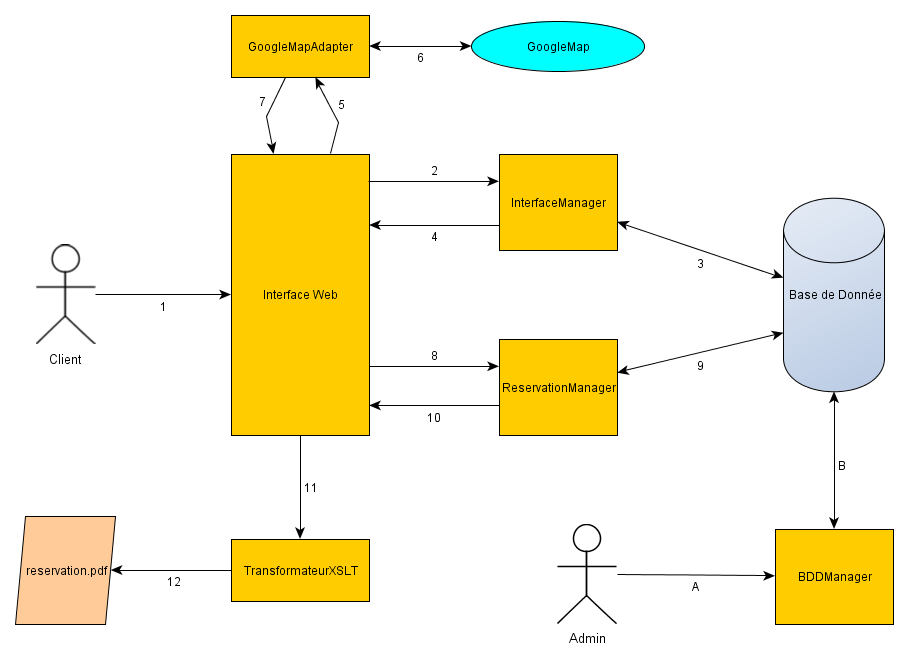
\includegraphics[width=1\textwidth]{overview}
			\label{overview}
		\end{figure}
		
	\section{Base de donnée}
		
		\begin{figure}[!h]
			\centering
			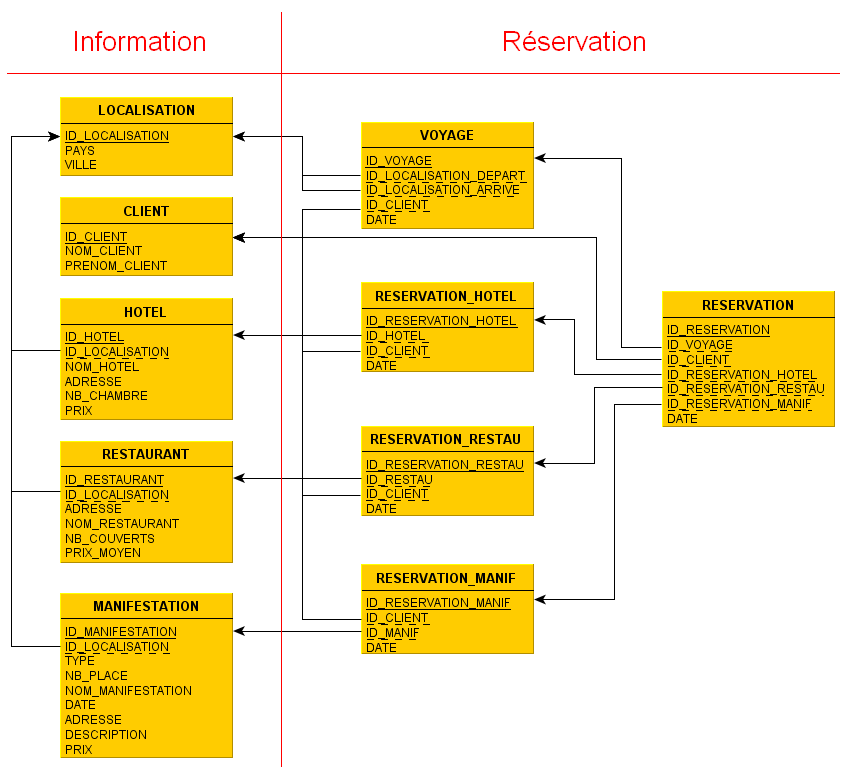
\includegraphics[width=1\textwidth]{bdd}
		\end{figure}
		
		Notre base de donnée contient deux types de tables :
		
		\begin{itemize}
		  \item Information, contenant les informations fixes de notre système. Elles
		  ne seront modifiables que par l'administrateur. 
		  \item Réservation, contenant les réservations faites par les clients.
		\end{itemize}
			
	\section{InterfaceWeb}
		
		L'interface consiste en un formulaire que le client va remplir
		(figure \ref{overview}, flèche 1 ) . A chaque modification du formulaire
		, il va se mettre à jour grâce au service InterfaceManager (figure
		\ref{overview}, flèches 2 et 4)
		
		Une fois toute les informations remplies, il est possible de visualiser les
		différentes adresses sur une carte, via un service GoogleMap (figure
		\ref{overview}, flèches 5 et 7)
		
		A la fin, le Client pourra valider sa réservation. Cela activera le service
		ReservationManager (figure \ref{overview}, flèches 8 et 10). Il enregistrera
		pour finir la réservation dans la Base de donnée, si possible, et retournera
		le résultat.
		
		Pour finir si la réservation est un succès, un résumé de celle-ci sera
		sauvegardé au format pdf (figure \ref{overview}, flèche 11).
	
	\section{InterfaceManager}
	
		\subsection{Fonctionnement}
	
			L'interfaceManager est un service qui récupère en entrée (figure
			\ref{overview}, flèche 2) toujours le méme format de donnée, et qui en
			fonction des champs plein ou vide recherchera dans la base de donnée
			(figure\ref{overview}, flèche 3) les information complémentaire, et les
			retournera à l'Interface (figure\ref{overview}, flèche 4).
		
		\subsection{Format des données}
		
			En entrée (figure\ref{overview}, flèche 2):
			\begin{itemize}
			  \item Pays
			  \item Ville
			  \item Date
			  \item Type de Manifestation\\
			\end{itemize}
			
			En sortie (figure\ref{overview}, flèche 4):
			\begin{itemize}
			  \item Pays
			  \item Villes
			  \item Type de Manifestations
			  \item Manifestations (Id,Nom,Adresse,Description,Prix,Places)
			  \item Hotels (Id,Nom,Adresse,Nombre de chambres,Prix)
			  \item Restaurants (Id,Nom,Adresse,Nombre de couvert,Prix moyen)
			\end{itemize}
		
		\subsection{Dépendances}
		
			Si le champs Pays de la requète est vide, InterfaceManager
			renvera la liste des pays contenues dans la base de donnée.
			
			Si le champs Pays est complété et que le champs Ville est vide,
			InterfaceManager renvera la liste des villes du pays spécifiée contenues dans
			la base de donnée.
		
			Si les champs Pays, Ville et Date sont complété et que le champs Type de
			Manifestations est vide, InterfaceManager renvera la liste des Type de
			Manifestations qui auront lieu dans cette Ville a cette Date.
			
			Enfin si tout les champs sont remplis InterfaceManager renvera la liste des
			Manifestation qui auront lieu dans cette Ville a cette Date et des Hotels et
			Restaurants de cette ville.
		
	\section{GoogleMapAdapter}	
		
		Grâce aux adresses des différents éléments de la réservation et en les
		envoyant(figure\ref{overview}, flèche 6) au service GoogleMap on
		recupère(figure\ref{overview}, flèche 7) une image que l'on ajoute au
		formulaire.
	
	\section{ReservationManager}	
	
		\subsection{Fonctionnement}
	
			Ce service sert à enregistrer, dans la base de données, les réservations
			choisis par le client. On lui envoie les Id de chaque élément à
			reserver(figure\ref{overview}, flèche 8), il vérifie que les reservations
			sont possible et si tout est OK il les éffectue(figure\ref{overview}, flèche
			9). Enfin il retourne un message confimant ou non la
			reservation(figure\ref{overview}, flèche 10).
	
		\subsection{Format des données}
		
			En entrée (figure\ref{overview}, flèche 8):
			\begin{itemize}
			  \item Nom
			  \item Prenom
			  \item IdManif
			  \item IdHotel
			  \item IdRestau
			  \item Voyage(Pays de Départ, Ville de Départ, Pays d'Arrivée, Ville de
			  d'Arrivée)\\
			\end{itemize}
	
			En sortie (figure\ref{overview}, flèche 10) une simple chaine de caractère.
	
	\section{TransformateurXSLT}
	
		L'interface envoie un fichier XML qui va etre transformer en fichier pdf grâce
		à un fichier xsl decrivant la transformation. 
	
	\section{BDDManager}
		
		
\clearpage
